\id{ҒТАМР 65.65.03}{https://doi.org/10.58805/kazutb.v.1.26-748}

\begin{articleheader}
\sectionwithauthors{М.Ч. Тултабаев, М. Султанова, Н. Акжанов, А. Сәдуакас}{МАҚСАРЫ МАЙЫ НЕГІЗІНДЕГІ ШПИНАТ ТҰЗДЫҒЫНЫҢ САҚТАУ ТҰРАҚТЫЛЫҒЫН ЗЕРТТЕУ}

{\bfseries
М.Ч. Тултабаев\textsuperscript{\envelope } \authorid,
М. Султанова\authorid,
Н. Акжанов\authorid,
А. Сәдуакас\authorid}
\end{articleheader}

\begin{affiliation}
\emph{«Қазақ қайта өңдеу және тағам өнеркәсіптері ҒЗИ» ЖШС АФ, Астана, Қазақстан,}

\raggedright \textsuperscript{\envelope }{\em Корреспондент-автор: shomanyli@mail.ru}
\end{affiliation}

Бұл мақалада мақсары майы негізінде шпинат тұздығының сақтау
тұрақтылығын анықтауға арналған зерттеу жұмыстары қарастырылды. Шпинат
құрамында A, C, K дәрумендері мен темір, магний сияқты минералдар бар,
олар иммунитетті нығайтуға ықпал етеді. Мақсары майы линол қышқылы мен
антиоксиданттарға бай, сонымен қоса жүрек-қан тамырлары жүйесіне пайдалы
әсер етеді. Тұздық дайындау процесі 85°C температурада шпинатты
бланштау, оны салқындату және паста тәрізді консистенцияға дейін
жеткізу, содан кейін май, лимон шырыны, сарымсақ және дәмдеуіштерді қосу
арқылы жүзеге асырылады. Тұздық сапасын бағалау үшін қышқылдық (pH
өлшегіш әдісі), ылғалдылық (құрғату әдісі) және май қышқылдары құрамына
(газды хроматография әдісі) талдау жүргізілді. Органолептикалық
сипаттамалар мен көрсеткіштер дегустациялық комиссиямен бағаланды.
Алынған тұздық жоғары тағамдық және функционалдық қасиеттерге ие, сақтау
кезінде тұрақты және сау тамақтануға ұсынылады. Ол шпинат пен мақсары
майының пайдалы компоненттерін біріктіріп, рационға құнды қосымша тағам
болып табылады. Дегустациялық сынақтар тұздықтың дәмдік сапасын жоғары
бағалауды көрсетіп қана қоймай, бұл оның тұтынушылар үшін тартымдылығын
растайды. Дайындалған шпинат тұздығы мақсары майы негізінде
функционалдық өнім болып табылады, күнделікті тамақтану рационын
жақсартуға және денсаулықты қолдау үшін жақсы ықпал етеді.

{\bfseries Түйін сөздер:} шпинат, мақсары майы, тұздық, физика-химиялық
қасиеттер, органолептикалық қасиеттер.

\begin{articleheader}
{\bfseries ИССЛЕДОВАНИЕ УСТОЙЧИВОСТИ ХРАНЕНИЯ ШПИНАТНОГО СОУСА НА ОСНОВЕ
САФЛОРОВОГО МАСЛА}

{\bfseries
М.Ч. Тултабаев\textsuperscript{\envelope },
М. Султанова,
Н. Акжанов,
А. Сәдуакас}
\end{articleheader}

\begin{affiliation}
\emph{АФ ТОО «Казахский НИИ перерабатывающей и пищевой промышленности», Астана, Казахстан,}

\emph{e-mail: shomanyli@mail.ru}
\end{affiliation}

В этой статье были рассмотрены исследовательские работы по определению
устойчивости хранения шпинатного соуса на основе сафлорового масла,
обладающего высокой пищевой ценностью. Шпинат является ценным источником
витаминов A, C, K и минералов, таких как железо и магний, способствующих
укреплению иммунитета. Сафлоровое масло богато линолевой кислотой и
антиоксидантами, что делает его полезным для сердечно-сосудистой
системы. Процесс приготовления соуса включал бланширование шпината при
85°C, его охлаждение и измельчение до пастообразной консистенции с
последующим добавлением масла, лимонного сока, чеснока и специй. Для
оценки качества соуса были проведены анализы кислотности ( метод
pH-метр), влажности (метод сушки) и жирнокислотного состава (метод
газовой хроматографии). Органолептические характеристики оценивались
дегустационной комиссией. Полученный соус обладает высокими питательными
и функциональными свойствами, стабильностью при хранении и может быть
рекомендован для здорового питания. Он сочетает в себе полезные
компоненты шпината и сафлорового масла, что делает его ценным
дополнением к рациону. Дегустационные испытания показали высокую оценку
вкусовых качеств соуса, что подтверждает его привлекательность для
потребителей. Разработанный шпинатный соус на основе сафлорового масла
представляет собой функциональный продукт, способствующий улучшению
рациона питания и поддержанию здоровья.

{\bfseries Ключевые слова:} шпинат, сафлоровое масло, соус,
физико-химические свойства, органолептические свойства.

\begin{articleheader}
{\bfseries INVESTIGATION OF THE SHELF LIFE OF SPINACH SAUCE BASED ON SAFFLOWER OIL}

{\bfseries
M.Ch. Tultabayev\textsuperscript{\envelope },
M. Sultanova,
N. Akzhanov,
A Saduakas}
\end{articleheader}

\begin{affiliation}
\emph{«Kazakh research Institute of processing and food industry» LLP AF, Astana, Kazakhstan,}

\emph{e-mail: shomanyli@mail.ru}
\end{affiliation}

This article reviewed research papers on determining the storage
stability of spinach sauce based on safflower oil, known for its high
nutritional value. Spinach is a rich source of vitamins A, C, K, and
minerals like iron and magnesium, which contribute to immune system
strengthening. Safflower oil is abundant in linoleic acid and
antioxidants, making it beneficial for cardiovascular health. The sauce
preparation process involved blanching spinach at 85°C, cooling it, and
blending it into a paste, followed by the addition of oil, lemon juice,
garlic, and spices. Quality assessments included acidity (pH meter),
moisture content (drying method), and fatty acid composition (gas
chromatography). Sensory characteristics were evaluated by a tasting
panel. The resulting sauce exhibits high nutritional and functional
properties, storage stability, and is recommended for healthy diets. It
combines the beneficial components of spinach and safflower oil, making
it a valuable addition to the diet. Sensory tests showed high ratings
for the sauce's taste qualities, confirming its appeal to consumers. The
developed spinach sauce based on safflower oil represents a functional
product that enhances dietary nutrition and supports health.

{\bfseries Keywords:} spinach, safflower oil, sauce, physicochemical
properties, organoleptic properties.

\begin{multicols}{2}
{\bfseries Кіріспе.} Өсімдік компоненттері негізіндегі тұздықтар
денсаулығына көңіл бөлетін тұтынушылар арасында танымалдылыққа ие болуда
{[}1{]}. Шпинат A, C, K витаминдері мен темір және магний сияқты
минералдарға бай, бұл оны адам рационында өте маңызды әрі қажетті өнімге
айналдырады. Ол иммунитетті нығайтуға және жалпы денсаулықты қолдауға
көмектеседі {[}2{]}.

Мақсары майы линол қышқылы мен антиоксиданттарға бай, бұл оны жүрек-қан
тамырлары ауруларының алдын алуда тиімді етеді {[}3{]}. Бұл
ингредиенттердің үйлесімі функционалдық өнім жасауға мүмкіндік береді,
ол тағамның дәмін жақсартып қана қоймай, оның тағамдық құндылығын да
арттырады {[}4{]}.

Дегенмен, өнімнің физика-химиялық және органолептикалық қасиеттерін,
сондай-ақ оның сақтау кезіндегі тұрақтылығын бағалау маңызды. Бұл
зерттеу қазіргі нарықтың талаптарына сай келетін, тұтынушыларды тек
жағымды дәмімен ғана емес, сонымен қатар пайдалы функционалдық
қасиеттерімен де қамтамасыз ететін мақсары майы негізіндегі шпинат
тұздығын әзірлеуге бағытталған {[}5{]}.

{\bfseries Материалдар мен әдістер.} Шпинат тұздығын әзірлеу үшін келесі
ингредиенттер пайдаланылды: Қазақстанда өсірілген шпинат (Spinacia
oleracea), мақсары майы, лимон шырыны, сарымсақ, тұз және дәмдеуіштер.
Шпинат A, C, K витаминдері мен темір, магний секілді минералдарға бай,
бұл жалпы денсаулықты сақтау үшін маңызды. Мақсары майы (Carthamus
tinctorius) ``КазИрАгро'' ЖШС (Жамбыл облысы, Қазақстан Республикасы)
компаниясынан алынған. Май бірінші суық сығымдау әдісімен алынған
тазартылған өнім болып табылады, құрамында линол қышқылының мөлшері
70\%-дан жоғары (өндірушінің мәліметі бойынша). Май +4 °C температурада
қараңғы жерде, герметикалық ыдыста сақталды, бұл оның тотығуынан
қорғайды.

Қосымша ингредиенттер ретінде лимон шырыны мен сарымсақ тұздықтың дәмдік
қасиеттерін жақсарту үшін қолданылды. Технологиялық процесс ГОСТ
31761-2012 және ГОСТ 31762-2012 стандарттарына сәйкес жүзеге асырылды.

Тұздық дайындау процесі бірнеше кезеңнен тұрды. Алдымен, жаңа шпинат
жапырақтары 85°C температурада қайнаған суда 3 минут бойы бланшталды,
бұл оның пайдалы заттарын және жарқын түсін сақтауға көмектесті {[}6{]}.
Бланштаудан кейін шпинат тез арада мұзды суға салынды. Содан соң,
салқындатылған шпинат блендермен ұсақталып пастаға айналды, бұл біртекті
текстураны қамтамасыз етті. Пастаға мақсары майы 1:0:2 қатынасында,
лимон шырыны, сарымсақ, тұз және дәмдеуіштер қосылып, бәрі мұқият
араластырылды, нәтижесінде біркелкі масса алынды {[}7{]}.

Тұздықтың физико-химиялық сипаттамаларын бағалау үшін келесі әдістер
қолданылды. Тұздықтың pH мәні рН-метр арқылы өлшеніп, қышқылдығы
анықталды, бұл тұздықтың сақтау мүмкіндігін бағалау үшін маңызды
көрсеткіш болып табылады. Тұздықтың ылғалдылығы 105°C температурада
тұрақты массаға дейін кептіру әдісімен анықталды, бұл осы типтегі
өнімдер үшін стандартты процедура {[}8{]}. Мақсары майының май қышқылы
құрамын газды хроматография әдісімен талдап, полиқанықпаған май
қышқылдары, оның ішінде линол қышқылының мөлшері анықталды, бұл оның
денсаулыққа пайдалы қасиеттерін растайды {[}9{]}.

Тұздықтың органолептикалық сипаттамалары, оның ішінде дәмі, иісі,
құрылымы және түсі дәм татушылармен 5 балдық шкала бойынша бағаланды,
мұнда 5 балл -- ең жоғары сапаны білдіреді. Тұздықтың тұрақтылығын
бағалау үшін өнім 4°C температурада 30 күн бойы сақталды. Ара-тұра (0,
10, 20 және 30 күндерде) pH өлшеніп, ылғалдылығы қайта анықталып,
органолептикалық бағалау жүргізілді, бұл тұздықтың сақтау барысында
қасиеттерінің өзгеруін анықтау мақсатында жүзеге асырылды {[}10{]}.

{\bfseries Нәтижелер мен талқылау.} Май қышқылдарының құрамын талдау
тағамдық құндылықты анықтау, функционалдық өнімдерді әзірлеу, сапа
бақылауын жүргізу және мақсары майының технологиялық қасиеттерін болжау
үшін қажет.

Мақсары майының май қышқылдары құрамы газды хроматография әдісімен
талданды. Нәтижелер көрсеткендей, майда линол қышқылының едәуір мөлшері
бар, ол полиқанықпаған май қышқылы болып табылады. Бұл мақсары майының
денсаулыққа пайдалы екенін, қандағы холестерин деңгейін төмендетуге және
жүрек-қан тамырлары жүйесінің қалыпты жұмысын қолдауға ықпал ететінін
растайды. Мұндай қасиеттер майды функционалдық өнімге айналдырып,
тұздықтың тұтынушылардың денсаулығына оң әсер етуі мүмкін (сурет 1).
\end{multicols}

{\bfseries 1 - сурет. Мақсары майының май қышқылдары құрамы}

\begin{multicols}{2}
Бұл диаграмма мақсары майында негізінен линол қышқылы (шамамен 70\%) бар
екенін көрсетеді, бұл оның полиқанықпаған май қышқылдарына жоғары
мөлшерде бай екенін айқындайды. Линол қышқылы өзінің пайдалы
қасиеттерімен танымал, мысалы, қандағы холестерин деңгейін қалыпты
ұстауға және жүрек-қан тамырлары жүйесінің жағдайын жақсартуға
көмектеседі.

Өнімнің негізі - мақсары майы, ол өзінің тұрақтандыратын қасиеттерімен
белгілі, бұл өнімнің сақтау барысында физикалық және химиялық
көрсеткіштерінің өзгерістеріне төзімділігін қамтамасыз етеді.

Өнімнің сапасының негізгі параметрлерінің бірі - pH деңгейі, ол
тұздықтың дәмдік қасиеттеріне, микробиологиялық тұрақтылығына және
сақтау мерзіміне әсер етеді. Зерттеу барысында шпинат тұздығының pH
деңгейі 30 күн бойы +4 °C температурада сақталған жағдайда өзгерісі
бақылауға алынды (кесте 1).
\end{multicols}

\begin{table}[H]
\caption*{1 - кесте. Мақсары майы негізіндегі шпинат тұздығының pH деңгейінің 30 күн бойы өзгерісі}
\centering
\begin{tblr}{
  row{1} = {c},
  cell{2}{1} = {c},
  cell{2}{2} = {c},
  cell{3}{1} = {c},
  cell{3}{2} = {c},
  cell{4}{1} = {c},
  cell{4}{2} = {c},
  cell{5}{1} = {c},
  cell{5}{2} = {c},
  cell{6}{1} = {c},
  cell{6}{2} = {c},
  hlines,
  vlines,
}
Сақтау күндері & pH  & Ескертпе                          \\
0күн           & 5.5 & Бастапқы pH көрсеткіші            \\
7күн           & 5.4 & pH деңгейінің аздап төмендеуі     \\
14күн          & 5.3 & pH деңгейінің төмендеуі жалғасуда \\
21күн          & 5.2 & pH деңгейінің жеңіл төмендеуі     \\
30күн          & 5.1 & pH деңгейінің минимальды өзгерісі 
\end{tblr}
\end{table}

\begin{multicols}{2}
Сақтау мерзімі ішінде тұздықтың рН деңгейі 6,1-ден 5,8-ге дейін
төмендеген. Бұл өзгеріс лимон шырынының табиғи органикалық қышқылдарының
әсерінен, сондай-ақ сақтау кезінде микробиологиялық процестердің
жүруімен байланысты. Сонымен, кесте 30 күн бойы сақтау барысында
тұздықтың pH деңгейінің минималды ауытқулармен тұрақты болғанын
көрсетеді. Бұл өнімнің сақтау кезінде жоғары тұрақтылығын дәлелдейді,
әрі оның сапасы мен қауіпсіздігін қамтамасыз ету үшін маңызды екенін
айқындайды.

Ылғалдылықтың аз өзгеруі өнімнің жақсы қаптамасымен және қолданылған
ингредиенттердің ерекшеліктерімен түсіндіріледі (кесте 2).
\end{multicols}

\begin{table}[H]
\caption*{2 - кесте. Мақсары майы негізіндегі шпинат тұздығының 30 күн бойы сақтау барысында ылғалдылығының өзгерісі}
\centering
\begin{tblr}{
  row{1} = {c},
  cell{2}{1} = {c},
  cell{2}{2} = {c},
  cell{3}{1} = {c},
  cell{3}{2} = {c},
  cell{4}{1} = {c},
  cell{4}{2} = {c},
  cell{5}{1} = {c},
  cell{5}{2} = {c},
  cell{6}{1} = {c},
  cell{6}{2} = {c},
  hlines,
  vlines,
}
Сақтау күндері & Ылғалдылық (\%) & Ескертпе                          \\
0күн           & 80              & Өнімнің бастапқы ылғалдылығы      \\
7күн           & 79              & Ылғалдылықтың шамалы төмендеуі    \\
14күн          & 78              & Ылғалдылықтың аздап төмендеуі     \\
21күн          & 77              & Ылғалдылықтың жеңіл төмендеуі     \\
30күн          & 76              & Ылғалдылықтың минималды төмендеуі 
\end{tblr}
\end{table}
\begin{multicols}{2}
Тәжірибе нәтижелері бойынша, сақтау мерзімі ішінде өнімнің ылғалдылығы
шамамен 4\%-ға төмендегені анықталды. Бұл өзгерістер өнімнің құрылымына
және органолептикалық қасиеттеріне әсер етті. Ылғалдың азаюы, негізінен,
май фазасының тұрақтылығына және сұйық фракцияның булануына байланысты
болып келеді.

Шпинат тұздығы жарқын дәмі, пайдалы қасиеттері мен функционалдық
құндылығын қамтамасыз ететін ингредиенттер негізінде әзірленді. Негізгі
компонент --- балғын шпинат, ол дәрумендер мен минералдардың бай көзі
болса, мақсары майы өнімді полиқанықпаған май қышқылдарымен байытады.
Лимон шырыны тұздыққа қышқылдық қосып, сарымсақ хош иісті күшейтеді, ал
дәмдеуіштер жалпы дәмдік үйлесімділікті толықтырады (кесте 3).
\end{multicols}

\begin{table}[H]
\caption*{3 - кесте. Мақсары майы негізінде шпинат тұздығының рецептурасы 100 г-100\%}
\centering
\begin{tblr}{
  cells = {c},
  hlines,
  vlines,
}
Ингредиенттер              & Құрамы, \% \\
Балғын шпинат              & 77,9       \\
Мақсары майы               & 15,4       \\
Лимон шырыны               & 3,8        \\
Сарымсақ                   & 1,7        \\
Тұз                        & 0,8        \\
Дәмдеуіштер (дәміне қарай) & 0,4        
\end{tblr}
\end{table}

\begin{multicols}{2}
Бұл рецептура шпинат тұздығына жоғары тағамдық құндылықты ғана емес,
сонымен қатар кең тұтынушылар тобына лайықты тартымды дәмді қамтамасыз
ететін теңдестірілген құрамды көрсетеді.

Органолептикалық сипаттамалар өнімнің дәмі, иісі, түсі және құрылымы
сияқты қасиеттерін сезім органдары арқылы қабылдауды сипаттайды. Мақсары
майы негізіндегі шпинат тұздығы үшін дәм тату сынақтары жүргізіліп,
нәтижелер өнімнің тұтынушылар үшін тартымдылығын көрсететін бағалар
түрінде ұсынылды (сурет 2).
\end{multicols}

\begin{figure}[H]
	\centering
	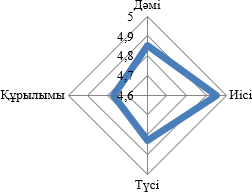
\includegraphics[width=0.5\textwidth]{media/pish3/image2}
	\caption*{2 - сурет. Мақсары майы негізіндегі шпинат тұздығының органолептикалық бағасы}
\end{figure}

\begin{multicols}{2}
Дәмі - баға 4.8 (соустың дәмі керемет, лимон шырынынан аздап қышқыл).

Иісі - баға 5.0 (жаңа, жарқын шпинат иісі, сарымсаққа тән иісі).

Түсі - баға 4.7 (жаңа шпинатқа тән қанық жасыл түс).

Құрылымы - баға 4.5 (ұнамды, жұмсақ, аздап кремді құрылым).

Профилограмма негізгі органолептикалық сипаттамалар бойынша бағалардың
таралуын айқын көрсетіп, өнімнің жалпы сапасын бағалауға мүмкіндік
береді.

Тұздық органолептикалық қасиеттері дәм тату арқылы бағаланып, жоғары
бағаларға ие болды. Соус жарқын жасыл түспен және жаңа шпинаттың бай хош
иісімен ерекшеленді. Дәмі теңдестірілген, лимон шырынынан келген жеңіл
қышқылдық және сарымсақтың ерекше хош иісі байқалады. Сапа шкаласы
бойынша бағасы 4-5 балл аралығында болды, бұл тұздықтың жоғары дәмдік
тартымдылығын растайды (сурет 3).
\end{multicols}

\begin{figure}[H]
	\centering
	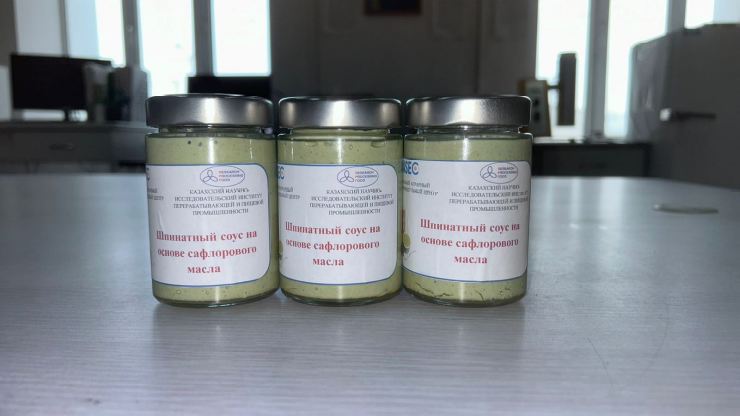
\includegraphics[width=0.8\textwidth]{media/pish3/image3}
	\caption*{3 - сурет. Мақсары майына негізделген шпинат тұздығы}
\end{figure}

\begin{multicols}{2}
Бұл нәтижелер басқа зерттеулердің деректерімен сәйкес келеді, олар
табиғи өсімдік компоненттерін, мысалы, шпинатты қамтитын тұздықтардың
жоғары органолептикалық сипаттамаларға ие болатынын және функционалдық
тамақ өнімдері нарығында сұранысқа ие болатынын көрсетеді.

\emph{Талқылау.} Алынған нәтижелерге сүйене отырып, шпинаттан жасалған
тұздық, мақсары майымен дайындалған, тек дәмді ғана емес, сонымен қатар
функционалдық қасиеттерге ие өнім болып табылады. Оның жақсы
физика-химиялық және органолептикалық қасиеттері бар. Мақсары майы,
полиқанықпаған май қышқылдарына бай, тұздықтың пайдалы қасиеттерін
жақсартады, ал шпинат қосымша витаминдер мен минералдармен байытады.
Тұздықтың тұрақтылығын бағалау оның 30 күн бойы сақталған кезде өз
қасиеттерін сақтайтынын көрсетті, бұл оны әртүрлі жағдайларда қолдануға
ыңғайлы етеді.

Сонымен қатар, бұл зерттеу нәтижелері мақсары майы негізінде әзірленген
шпинат тұздығы - денсаулықты қолдауға бағытталған функционалды өнімдер
нарығында сұранысқа ие болатынын растады. Линол қышқылы мен В тобының
витаминдерін қамтитын мұндай өнімдер өз денсаулығына мән беретін және
тамақтың қоректік құндылығын арттыруға ұмтылатын адамдар үшін маңызды
тағамдық қосымша бола алады.

{\bfseries Қорытынды.} Әзірленген шпинат тұздығы --- бұл жаңа шпинаттың
пайдалы қасиеттері мен жоғары сапалы мақсары майының тамаша үйлесімі.
Шпинатты өңдеудің дұрыс технологиялары, атап айтқанда бланштау, оның
құрамындағы витаминдер мен минералдарды сақтау және тұздықтың
органолептикалық қасиеттерін жақсартуға мүмкіндік берді. Алынған
нәтижелер мақсары майының құрамында негізінен линол қышқылы (шамамен
70\%) барын және оның полиқанықпаған май қышқылдарына бай екендігін
көрсетті. Линол қышқылы өзінің пайдалы қасиеттерімен танымал, ол қан
холестеринінің деңгейін қалыпты ұстауға және жүрек-қан тамырлары
жүйесінің денсаулығын жақсартуға ықпал етеді.

Тұздықтың өндірілу кезіндегі ылғалдылығы 80\% құрады. 30 күндік сақтау
барысында ылғалдылық тек 4\%-ға ғана төмендеді. Бұл тұздықтың
тұрақтылығын және оны ұзақ уақыт бойы сақтауға жарамды екенін
дәлелдейді. Ылғалдылықтың өзгеруінің аздығы жақсы қаптаманың әсерінен
болуы мүмкін, ол өнімдегі ылғалды сақтауға көмектеседі, сондай-ақ
қолданылған ингредиенттердің табиғи қасиеттері де осыған ықпал еткен
болуы мүмкін. Органолептикалық деректерге сүйенсек, тұздық ашық жасыл
түспен және жаңа шпинаттың бай хош иісімен ерекшеленеді. Оның дәмі жақсы
теңдестірілген, лимон шырынының жеңіл қышқылдығы мен сарымсақтың хош
иісі айқын байқалады. Сапа шкаласы бойынша бағасы 4-5 балл аралығында
болды, бұл тұздықтың жоғары дәмдік қасиеттерін көрсетеді.

{\bfseries Қаржыландыру:} Жұмыс Қазақстан Республикасының Ауыл шаруашылығы
министрлігі BR 22886613 "Ауыл шаруашылығы Өсімдік шаруашылығы өнімдері
мен шикізатын қайта өңдеу және сақтау жөніндегі инновациялық
технологияларды әзірлеу" қаржыландыратын бағдарлама шеңберінде
жүргізілді.

\emph{Қорытындылай келе, біз осы ғылыми жобаның барлық қатысушыларына
эксперименттік зерттеулер жүргізуге көмектескені үшін шын жүректен алғыс
айтқымыз келеді. Біз сондай-ақ "ҚазҒЗИ қайта өңдеу және тамақ
өнеркәсібі" ЖШС Астана филиалының басшылығы мен ғалымдарына алғысымызды
білдіреміз.}
\end{multicols}

\begin{center}
{\bfseries Әдебиттер}
\end{center}

\begin{references}
1. Лейберова, Н. В., and Л. А. Донскова Применение рыжикового масла в
рецептуре соуса на растительной основе // Индустрия питания/Food
Industry. -2018. --Т. 3. -№ 4. --С. 25-29. DOI
10.29141/2500-1922-2018-3-4-2

2. Давлатова М. С., Кароматов И. Д. Научные исследования лекарственных
свойств шпината //Биология и интегративная медицина. - 2017. -№. 10.
-С. 125-136.

3. Устенова Г. О., Тургумбаева А. А., Кантуреева А. Применение и свойства
сафлора красильного //Вестник Казахского Национального медицинского
университета. -2016. -№. 1. -С. 535-537.

4. Колногоров К.П. и др. Новые функциональные пищевые масложировые
продукты со сбалансированным жирнокислотным составом //Труды БГТУ.
Серия 2: Химические технологии, биотехнология, геоэкология. -- 2016.
-- №. 4 (186). -- С. 188-194.

5. Rahnama A., Farshad S., Ф., Moosa Meskarbashee, et.al. High
temperature perturbs physicochemical parameters and fatty acids
composition of safflower (Carthamus tinctorius L.) // BMC Plant Biol.
-2024. -Vol. 24(1). DOI
\href{https://doi.org/10.1186/s12870-024-05781-3}{10.1186/s12870-024-05781-3}

6. Tedom W. D. et al. Optimal conditions of steam blanching of spinach
(Spinacia oleracea), a leafy vegetable consumed in Cameroon
//International Journal of Nutritional Sciences and Food Technology.
-2020. -- Vol. 6(3). -P. 1-8.

7. Grzeszczuk M., Jadczak D., Podsiadło C. The effect of blanching,
freezing and freeze-storage on changes of some chemical compounds
content in New Zealand spinach //Journal of Fruit and Ornamental Plant
Research. -2007. --Vol. 66(1). -- P. 95-103. DOI
10.2478/v10032-007-0012-x

8. Давыдова У.Ю., Величко Н.А. Изменение качества майонезного соуса в
процессе хранения //Вестник Красноярского государственного аграрного
университета. -- 2017. -- №. 6. -- С. 85-90.

9. Турина Е. Л., Прахова Т. Я., Ефименко С. Г. Жирнокислотный состав
сортов сафлора в зависимости от региона возделывания //Международный
сельскохозяйственный журнал. -- 2023. -- №. 3. -- С. 287-291. DOI
10.55186/25876740\_2023\_66\_3\_287

10. Мухаметов А.Е., Аскарбеков Э.Б., Ербулекова М.Т., Сейсеналы М.Е.
Өсімдік майларының қоспасынан дайындалатын майлы өнімдердің сапалық
көрсеткіштерін зерттеу // Алматы технологиялық университетінің
хабаршысы. -2022. -№ (4). --Б. 61-68. DOI
10.48184/2304-568X-2022-4-61-68
\end{references}

\begin{center}
{\bfseries References}
\end{center}

\begin{references}
1. Lejberova, N. V., and L. A. Donskova Primenenie ryzhikovogo masla v
recepture sousa na rastitel' noj osnove // Industrija
pitanija/Food Industry. -2018. --T. 3. -№ 4. --S. 25-29. DOI
10.29141/2500-1922-2018-3-4-2

2. Davlatova M. S., Karomatov I. D. Nauchnye issledovanija lekarstvennyh
svojstv shpinata //Biologija i integrativnaja medicina. - 2017. -№. 10.
-S. 125-136. {[}in Russian{]}

3. Ustenova G. O., Turgumbaeva A. A., Kantureeva A. Primenenie i
svojstva saflora krasil' nogo //Vestnik Kazahskogo
Nacional' nogo medicinskogo universiteta. -2016. -№. 1.
-S. 535-537. {[}in Russian{]}

4. Kolnogorov K.P. i dr. Novye funkcional' nye pishhevye
maslozhirovye produkty so sbalansirovannym zhirnokislotnym sostavom
//Trudy BGTU. Serija 2: Himicheskie tehnologii, biotehnologija,
geojekologija. -- 2016. -- №. 4 (186). -- S. 188-194. {[}in Russian{]}

5. Rahnama A., Farshad S., F., Moosa Meskarbashee, et.al. High
temperature perturbs physicochemical parameters and fatty acids
composition of safflower (Carthamus tinctorius L.) // BMC Plant Biol.
-2024. -Vol. 24(1). DOI 10.1186/s12870-024-05781-3

6. Tedom W. D. et al. Optimal conditions of steam blanching of spinach
(Spinacia oleracea), a leafy vegetable consumed in Cameroon
//International Journal of Nutritional Sciences and Food Technology.
-2020. -- Vol. 6(3). -P. 1-8.

7. Grzeszczuk M., Jadczak D., Podsiadło C. The effect of blanching,
freezing and freeze-storage on changes of some chemical compounds
content in New Zealand spinach //Journal of Fruit and Ornamental Plant
Research. -2007. --Vol. 66(1). -- P. 95-103. DOI
10.2478/v10032-007-0012-x

8. Davydova U.Ju., Velichko N.A. Izmenenie kachestva majoneznogo sousa v
processe hranenija //Vestnik Krasnojarskogo gosudarstvennogo agrarnogo
universiteta. -- 2017. -- №. 6. -- S. 85-90. {[}in Russian{]}

9. Turina E. L., Prahova T. Ja., Efimenko S. G. Zhirnokislotnyj sostav
sortov saflora v zavisimosti ot regiona vozdelyvanija //Mezhdunarodnyj
sel' skohozjajstvennyj zhurnal. -- 2023. -- №. 3. -- S.
287-291. DOI 10.55186/25876740\_2023\_66\_3\_287 {[}in Russian{]}

10. Mýhametov A.E., Askarbekov E.B., Erbýlekova M.T., Seısenaly M.E.
Ósimdik maılarynyń qospasynan daıyndalatyn maıly ónimderdiń sapalyq
kórsetkishterin zertteý // Almaty tehnologıalyq ýnıversıtetiniń\\
habarshysy. -2022. -№ (4). --Б. 61-68. DOI
10.48184/2304-568X-2022-4-61-68 {[}in Kazakh{]}
\end{references}

\begin{authorinfo}
\emph{{\bfseries Авторлар туралы мәліметтер}}

Тултабаев М.Ч- техника ғылымдарының докторы, «Қазақ қайта өңдеу және
тағам өнеркәсіптері ғылыми-зерттеу институты» ЖШС Астана филиалының жоба
жетекшісі, Астана, Қазақстан, e-mail: shomanyli@mail.ru;

Султанова Мю- техника ғылымдарының магистрі, «Қазақ қайта өңдеу және
тағам өнеркәсіптері ғылыми-зерттеу институты» ЖШС Астана филиалының жоба
жетекшісі, Астана, Қазақстан, e-mail: sultanova.2012@mail.ru;

Акжанов Н.-жаратылыстану ғылымдары магистрі, «Қазақ қайта өңдеу және
тағам өнеркәсіптері ғылыми-зерттеу институты» ЖШС Астана филиалының аға
ғылыми қызметкері, Астана, Қазақстан, e-mail: nurtore0308@gmail.com;

Садуакас А.-«Қазақ қайта өңдеу және тағам өнеркәсіптері ғылыми-зерттеу
институты» ЖШС Астана филиалының өсімдік шикізатын бастапқы өңдеу
зертханасының ғылыми қызметкері, Астана, Қазақстан, тe-mail:
aykon96@mail.ru.

\emph{{\bfseries Information about the authors}}

Tultabayev M.Ch.- Doctor of Technical Sciences, Project Manager of the
Astana branch of the Kazakh Research Institute of Processing and Food
Industries LLP, Astana, Kazakhstan, e-mail: shomanyli@mail.ru;

Sultanova M.-Master of Technical Sciences, Project Manager of the Astana
Branch of the Kazakh Research Institute of Processing and Food
Industries LLP, Astana, Kazakhstan, e-mail:
\href{mailto:sultanova.2012@mail.ru}{\nolinkurl{sultanova.2012@mail.ru}};

Akzhanov N.-Master of Natural Sciences, Senior Researcher of the Astana
Branch of the Kazakh Research Institute of Processing and Food
Industries LLP, Astana, Kazakhstan, e-mail: nurtore0308@gmail.com;

Saduakas A.- Researcher of the Laboratory of Primary Processing of Plant
Raw Materials, Astana Branch of the Kazakh Research Institute of
Processing and Food Industries, Astana, Kazakhstan, e-mail:
aykon96@mail.ru.
\end{authorinfo}
